\documentclass[french]{article}

\usepackage{MyPack2}
\geometry{top=2cm, bottom=2cm, left=3cm, right=3cm}
\title{\bsc{SIG} 1}
\author{Binôme A11 \\ \bsc{Simon} Léo, \bsc{Levy--Falk} Hugo}
\date{\today}

\begin{document}
\maketitle

\tableofcontents
\listoffigures
\newpage

\initPage{TL - SIG1}{\today}{\bsc{Simon}, \bsc{Levy--Falk}}

\part{Opérations de base sur les signaux}

\section{Signal numérique de synthèse}

Notre objectif  est de définir quelques fonctions de calcul de base sur les signaux afin de découvrir les outils de Matlab.

\subsection{Génération du signal}

Tout d'abord, nous avons cherché à générer un signal sinusoïdal et à l'échantillonner avant de tracer son graphe. Après avoir effectué quelques tracés, nous avons également pu mettre en évidence le théorème de Niquist-Shannon. La figure \ref{signalSin} montre le résultat obtenu pour une fréquence d'échantillonage de 50 Hz, une fréquence de 4 Hz et N=25.

\begin{figure}[h!]
\centering
\includegraphics{images/signalSinus.eps}
\caption{Signal sinusoïdal généré.}
\label{signalSin}
\end{figure}

\subsection{ Énergie et puissance}

Dans le but de calculer l'énergie d'un signal sans utiliser \verb`for`, nous avons effectué un produit terme à terme et utilisé l'outil \verb`sum`. Une manière encore plus efficace de procéder aurait été de réaliser le produit entre le vecteur donné en entrée et sa transposée. Nous avons ensuite calculé la puissance moyenne de manière théorique, en utilisant l'identité :

\[
\sin^2(x)=\frac {1-\cos(2x)} {2}
\]

on obtient
\[
\frac{1} {2 \pi} \int_{0}^{2 \pi} \sin^2(x) \mathrm{d}x = 1/2
\]

Par ailleurs, nous avons estimé la puissance de notre signal en utilisant la fonction puissance qui effectue la somme du produit terme à terme du signal et divise par la longueur de ce signal.

\lstset{language=matlab}
\begin{lstlisting}
>> s = sig1_sinus(4, 50, 2*50/4);
>> puissance(s)

ans =

    0.5000
\end{lstlisting}

On obtient un résultat conforme au calcul réalisé.

\subsection{ Quantification}

Pour quantifier un signal sur N bits, on commence par le centrer en 0 et le borner entre -0.5 et 0.5 à l'aide d'une première homothétie. Soit $s_1$ le signal ainsi obtenu. On réalise ensuite la quantification. Si $N > 0$ est le nombre de bit de quantification, on pose $q=\frac{1}{2^N}$. Dans un premier temps, on pose $s_2$ tel que :
\[
  s_2[k] = (\lfloor \frac{s_1[k]}{q} \rfloor + \frac{1}{2}) \times q
\]

Cependant cette formule est problématique pour la valeur maximale atteinte par la fonction. En effet, on a alors :
\[
s_2[k] = ( \lfloor \frac{1}{2q} \rfloor + \frac{1}{2}) \times q ) = (2^{N-1} + \frac{1}{2}) \times \frac{1}{2^N} > \frac{1}{2}
\]

Ce qui est incohérent avec le signal original. Une solution est de poser :
\[
  s_2[k] = min((\lfloor \frac{s_1[k]}{q} \rfloor + \frac{1}{2}) \times q, \frac{1}{2} - \frac{q}{2})
\]

Il ne reste plus qu'à remettre la fonction à l'échelle. On obtient le code suivant :

\lstset{language=matlab}
\begin{lstlisting}
function sig_quant = quantifie(X, n_bit)
    m = min(X);
    M = max(X);
    c = (m+M)/2;
    d = M-m;
    q = 1 / (2 ^ n_bit);
    s1 = (X - c)/d;
    sig_quant = min((floor(s1/q) + 1/2) * q, 1/2-q/2)*d + c;
end
\end{lstlisting}
En appliquant la fonction \verb`quantifie` pour $N=3$ et $N=8$ à un signal généré grâce à la fonction écrite dans la partie 1, on obtient la figure \ref{signalBruit}. On peut noter qu'il est difficile de différencier le signal d'entrée du signal quantifié sur 8 bits. La figure \ref{signalBruit2} montre offre un zoom qui permet de différencier le signal de la quantification.

\begin{figure}[h!]
\centering
\includegraphics{images/signalBruit.eps}
\caption{Quantification du signal sinusoïdal généré.}
\label{signalBruit}
\end{figure}
\begin{figure}[h!]
	\centering
	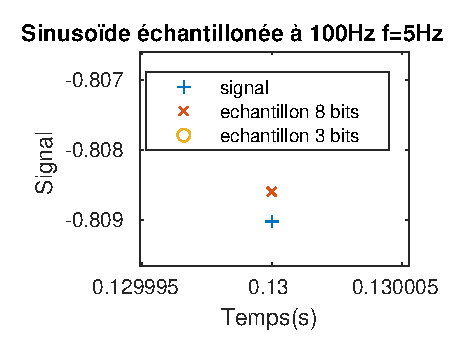
\includegraphics{images/signalBruit1.eps}
	\caption{Quantification du signal sinusoïdal généré - zoom.}
	\label{signalBruit2}
\end{figure}

%\FloatBarrier

Pour déterminer le bruit de quantification, on calcule la différence entre le signal d'origine et le signal quantifié, et on en détermine l'énergie. On calcule également la valeur théorique du bruit de quantification. On obtient

\begin{itemize}
	\item pour 8 bits, $4.6464 \times 10^{-6}$, pour une valeur théorique de $1.272 \times 10^{-6}$;
	\item pour 3 bits, $0.0063$, pour une valeur théorique de $0.0013$.
\end{itemize}

On remarque que l'échantillonnage à 8 bits est bien plus efficace, bien que la valeur théorique soit plus faible que celle calculée.

\section{ Signal audio}

\subsection{ Restitution}

En écoutant le signal enregistré à différentes fréquences de restitutions, on remarque que augmenter cette fréquence diminue la durée de la restitution et décale les fréquences de l'enregistrement vers des fréquences plus hautes. Inversement, diminuer la fréquence de restitution augmente la durée de l'enregistrement tout en déplaçant les fréquences des sons de l'enregistrement vers les graves.

\subsection{ Quantification}

A l'aide de la fonction \verb`quantifie` réalisée dans la partie précédente, on réalise la quantification du signal enregistré. On observe que plus le nombre de bits de quantification est faible, plus le bruit (à l'écoute) est important.

Les figures \ref{sonQuantifie1} et \ref{sonQuantifie2} donnent une représentation graphiques de différentes quantification du signal vocal.

\begin{figure}[!htbp]
\centering
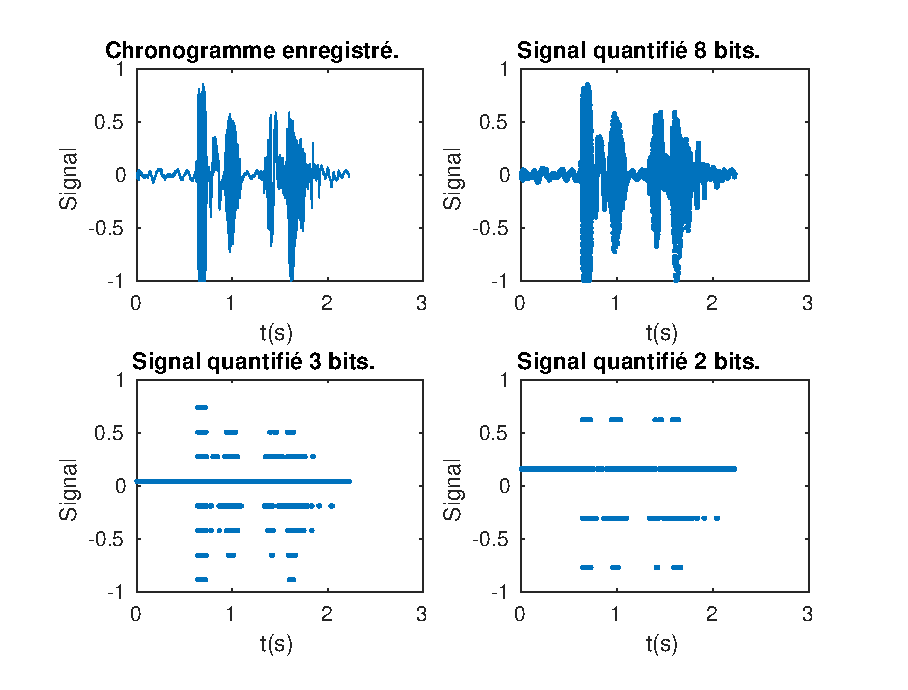
\includegraphics[width=\textwidth]{images/sonQuantifie2.eps}
\caption{Quantification du signal vocal enregistré.}
\label{sonQuantifie1}
\end{figure}

\begin{figure}[!htbp]
\centering
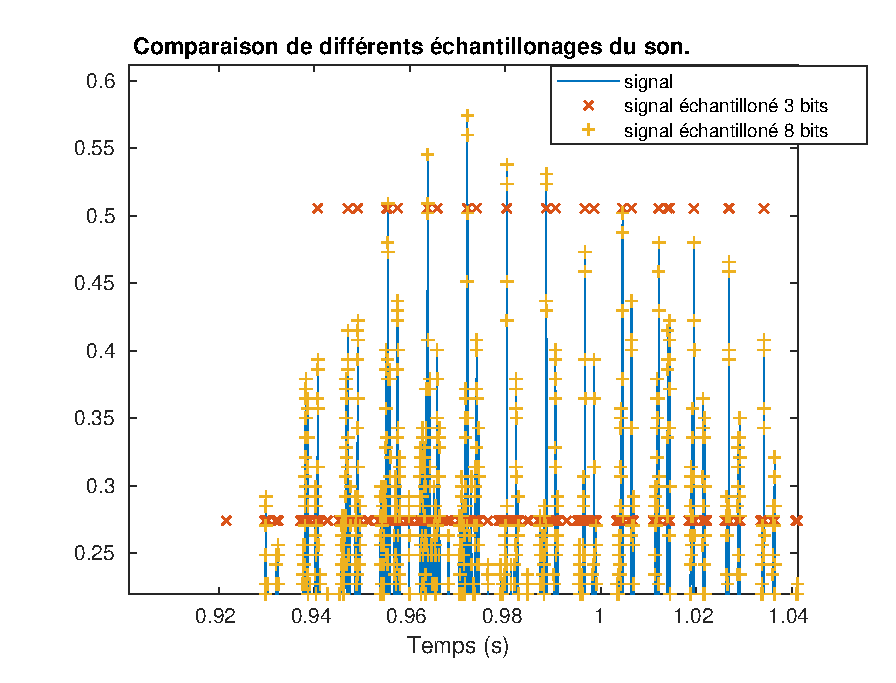
\includegraphics[width=\textwidth]{images/sonQuantifie.eps}
\caption{Quantification du signal vocal enregistré - comparaison en zoom.}
\label{sonQuantifie2}
\end{figure}

%\FloatBarrier
\newpage
\part{ Classification des signaux}

\section{ Exemple de calcul théorique}

Pour le signal $y(t) = A \sin(2 \pi f t)$ on a :

\[
\gamma_y(\tau) = \int_0^{\frac{1}{f}} A^2 \sin(2\pi f t) \sin(2 \pi f (t+\tau)) dt \
= \frac{A^2}{2f} \cos 2\pi f \tau - \frac{A^2}{2}\int_0^{\frac{1}{f}} \cos (2 \pi f (2t + \tau)) dt
\]

On obtient la fonction d'autocorrélation suivante :
\[
\gamma_y (t) = \frac{A^2} {2f} cos(2 \pi f t)
\]

\section{ Programmation}

On calcule l'autocorrélation avec la formule suivante :

\[
\gamma_x [n] = \sum_{k = 0} ^{length (x)} x[k]x[k+n]
\]

\begin{figure}[h!]
	\centering
	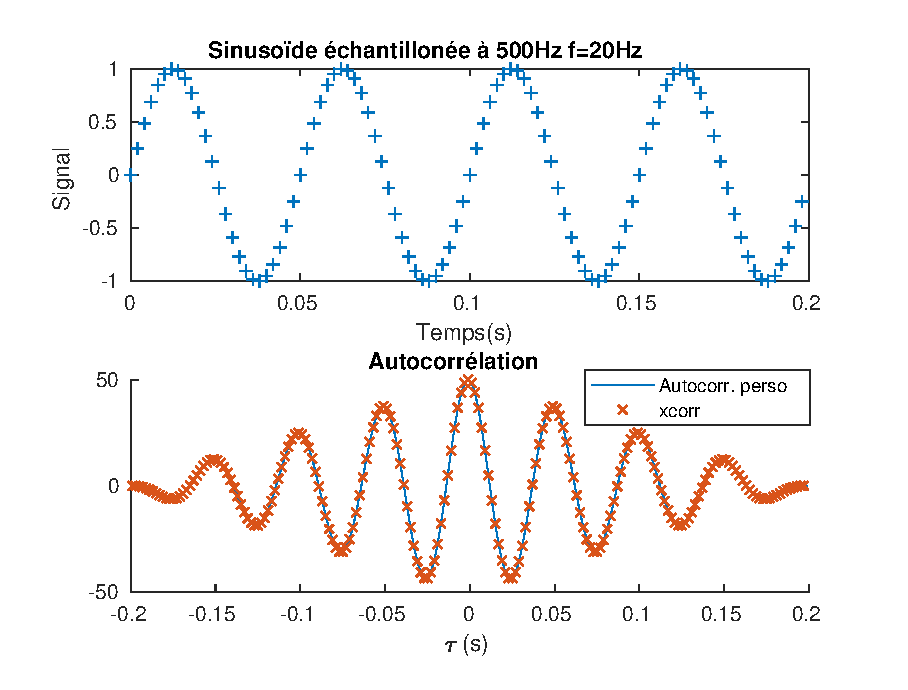
\includegraphics{images/autocorr.eps}
	\caption{Comparatif de de la fonction xcorr et de notre implémentation de l'autocorrélation.}
	\label{autocorr}
\end{figure}

La figure \ref{autocorr} montre que le résultat de \verb`xcorr` et de notre implémentation de l'autocorrélation sont identiques.

Nous n'avions d'abord tracé que la partie positive, avant de nous rendre compte de la nécessité de tracer également la partie négative.
On obtient un résultat du résultat théorique car le support de notre signal est fini, ce qui donne un cosinus amorti de manière symétrique et non un simple cosinus.

\section{ Application à la classification de quelques signaux simples}

Lorsque le signal se "répète" au cours du temps son autocorrélation est semblable sur de courtes périodes (reproduction du même motif au cours des périodes), on dit alors que le signal est stationnaire. Par contre si son autocorrélation est presque nulle, cela veut dire qu'il n'y a pas reproduction des motifs au cour des périodes et donc que le signal est non stationnaire.

\begin{figure}[h!]
	\centering
	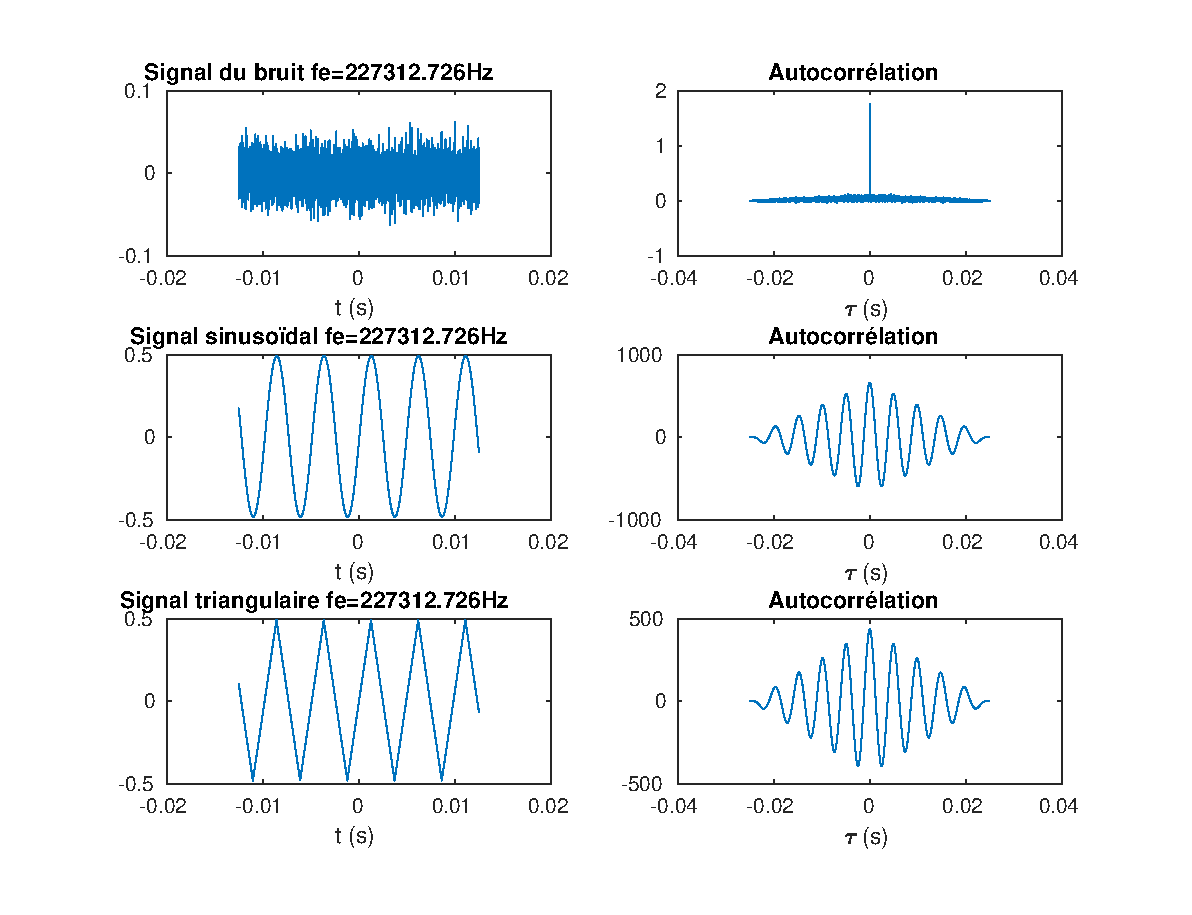
\includegraphics[width=1\textwidth]{images/classificationSig.eps}
	\caption{Autocorrélation de plusieurs signaux.}
	\label{classifSig}
\end{figure}

La figure \ref{classifSig} montre que les signaux sinusoïdaux et triangulaires sont stationnaires, contrairement au signal du bruit.

\begin{figure}[h!]
\centering
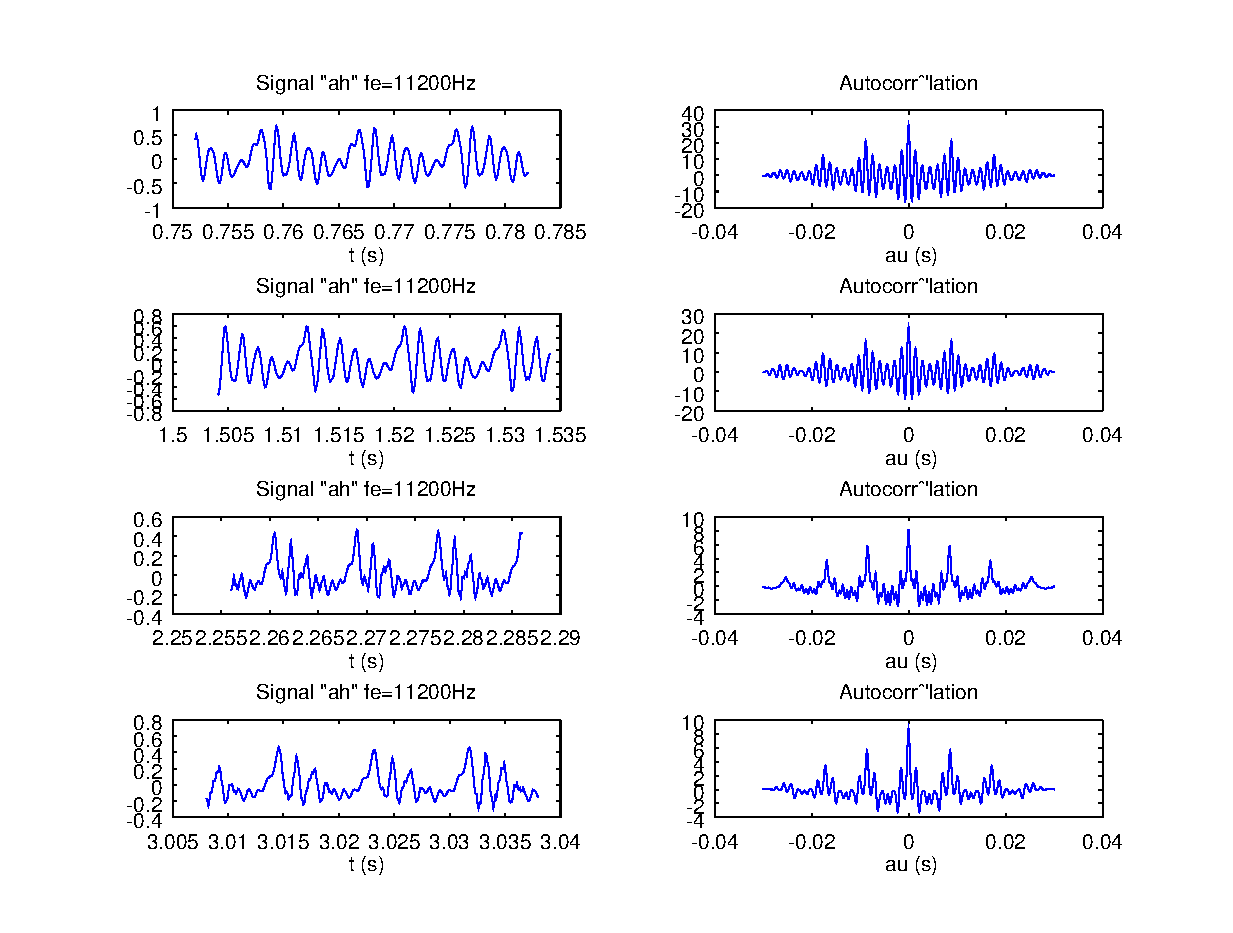
\includegraphics[width=\textwidth]{images/classificationAh.eps}
\caption{Autocorrélation de divers échantillons du signal vocal.}
\label{classifAh}
\end{figure}

La figure \ref{classifAh} montre que le signal vocal est quasi-stationnaire. En effet, sur de courtes périodes, son autocoorélation varie peu. ces résultats vont nous permettre dans la section suivante de séparer les différentes composantes d'un signal vocal. En effet, celles constituées essentiellement de bruit présenterons une autocorrélation très faible devant celles des parties voisées.

\FloatBarrier

\section{ Classification de signaux de parole voisés ou non voisés}

D'après les résultats de la section précédente, on peut différencier un signal de parole voisé d'un non voisé en visualisant l'autocorrélation. En effet un signal non voisé est constitué de bruit et devrait présenter une autocorrélation faible, et non périodique. Se pose alors la question de la longueur des échantillons sur lesquels on calcule l'autocorrélation. Nous avons essayé les durées 0.01, 0.06, 0.16 et 0.64 secondes.

\begin{figure}[h!]
\centering
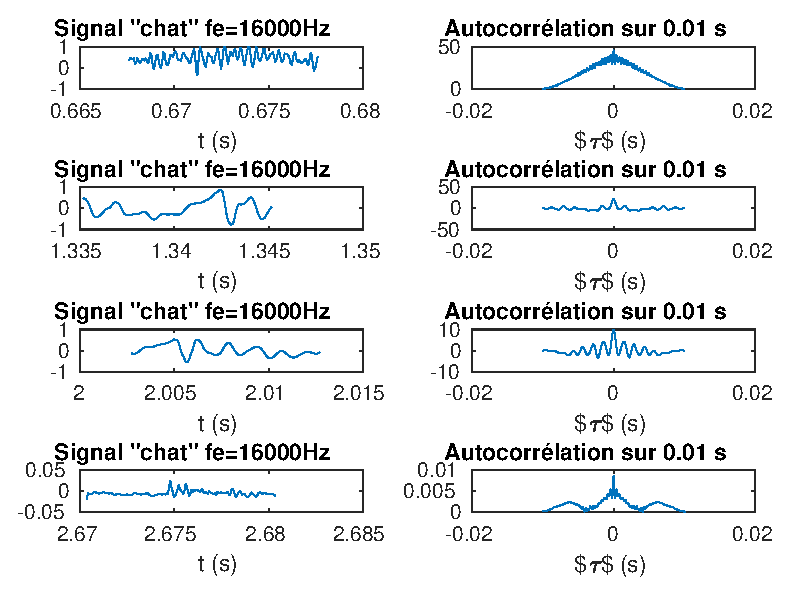
\includegraphics[width=\textwidth]{images/classificationVoix1.eps}
\caption{Autocorrélation de divers échantillons du signal vocal.}
\label{classif1}
\end{figure}

La figure \ref{classif1} montre que des échantillons de durée 0.01 secondes sont trop courts pour différencier aisément le signal voisé du non voisé.

\begin{figure}[h!]
\centering
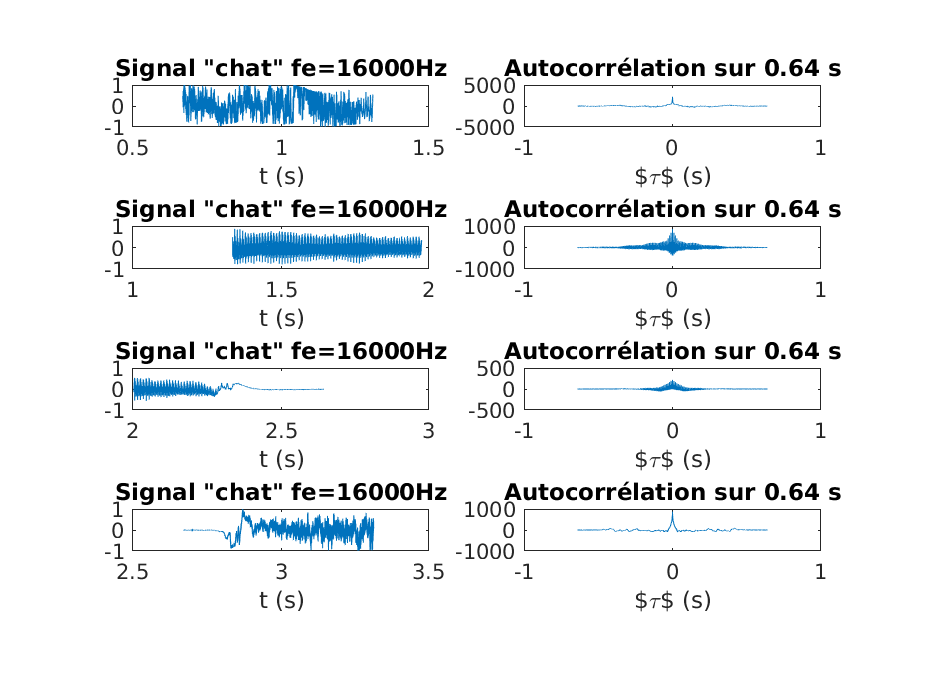
\includegraphics[width=\textwidth]{images/classificationVoix4.eps}
\caption{Autocorrélation de divers échantillons du signal vocal.}
\label{classif4}
\end{figure}

La figure \ref{classif4} montre que des échantillons de durée 0.64 secondes sont trop longs. En effet, on se rapproche alors de la période de variation du signal liée au sens de la parole (visible sur l'échantillon pris entre 2 et 2.8 secondes par exemple).


Finalement,  on choisit une durée d'échantillon de 0.16 secondes (figure \ref{classif3}), car bien que celle de 0.06 convienne également pour différencier le signal voisé du non voisé, l'autocorrélation sur une plus grande période fait apparaître plus de maximums locaux, ce qui permet d'estimmer plus précisément la fréquence fondamentale du signal voisé. On trouve ainsi une fréquence du fondamental de 100 Hz environ.

\begin{figure}[h!]
	\centering
	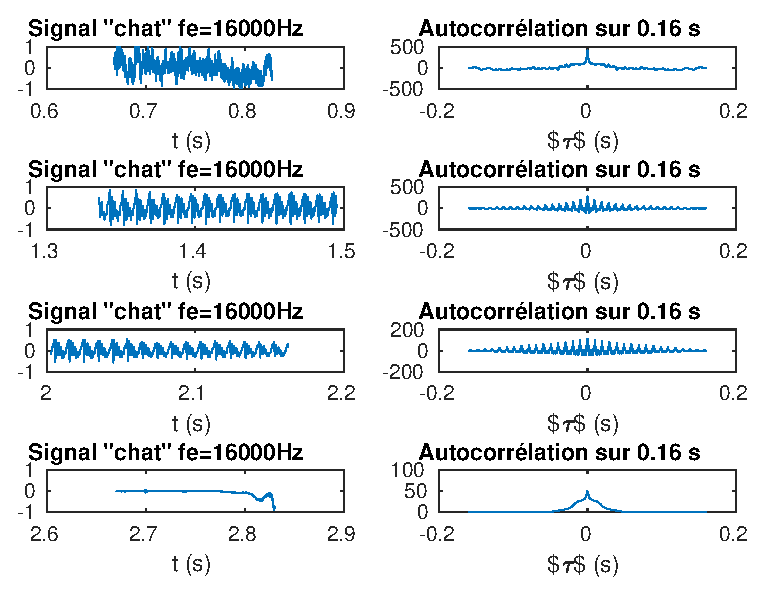
\includegraphics[width=\textwidth]{images/classificationVoix3.eps}
	\caption{Autocorrélation de divers échantillons du signal vocal.}
	\label{classif3}
\end{figure}

\end{document}
